\chapter{Methodology} \label{sec:methodology}

As summarized by the survey paper \cite{nid_ml_survey_2019} of Hongyu Liu and Bo Lang in section \ref{section:stateofart:nid_machine_learning_survey}, the design space for \gls{ml} based \gls{nids} is vast and can be hard to navigate at times. Hence, careful consideration of data representation, data pre-processing, \gls{ml} models, model parameters and training hyperparameters is necessary. The goal of the thesis was to examine the benefit of pre-training for already established \gls{dl} models in the context of \gls{nids}, hence we wanted to start from the most effective \gls{dl} models available, which, derived from state-of-the-art research, seems to be a uni-directional multi-layer \gls{dlstm} network. Additionally, we also looked at research on \gls{dl} and self-supervised/unsupervised learning in general. Most of the state-of-the-art research on \gls{dl}, and especially in self-supervised/unsupervised and transfer learning, is done in the context of \gls{nlp} \cite{bert}, \cite{elmo}, \cite{attention}.

Network communication is similar to natural language in the sense that it follows a certain set of rules, a grammar so to say, and each token like a word or packet conveys some semantic meaning when in the context of a sentence or flow. Other researchers have made similar observations \cite{anomaly_detection_recurrent_neural_networks}. We deemed the TransformerEncoder, which is often cited as an advancement of the \gls{lstm} in sequence modeling, to be a powerful new tool for network traffic classification. 

\section{Datasets} \label{sec:methodology:datasets}

We used the two \gls{nids} datasets \textit{UNSW-NB15} \cite{unsw_nb15} and \textit{CIC-IDS-2017} \cite{cic_ids_2017}. \par

\subsection{UNSW-NB15} \label{sec:methodology:datasets:unsw_nb15}

The UNSW-NB15 dataset \cite{unsw_nb15}, created by Nour Moustafa et al. from the School of Engineering and Information Technology, University of New South Wales at the Australian Defence Force Academy, Australia, was released as an update for the formerly frequently used but deprecated \cite{unsw_nb15} KDD dataset family. It was designed to reflect most known low foot print attacks at time of publication. The records are bidrectional flows extracted from the raw traffic data and grouped by the commonly used \textit{<srcIP, dstIP, srcPort, dstPort, protocol>} tuple. Each flow is described by 47 derived or measured features e.g. total duration, bytes transmitted, the mean of the flow packet size transmitted by destination IP, etc. The dataset contains a total of 2.54 million records of which 2.22 million are natural transaction data labeled as benign and 0.32 million attack records meaning 87.4\% of data is classified as benign. Attack records can be further divided into nine attack categories as listed in table \ref{table:methodology:datasets:unsw_nb15_categories}.

\begin{table}[H]
	\centering
	\begin{tabular}{c c c c c}
			\thead{\textbf{Type}} & \thead{\textbf{\textbf{No. Records}}} & \thead{\textbf{\% w.r.t.} \\ \textbf{majority class}} & \thead{\textbf{\% w.r.t.} \\ \textbf{majority attack class}} & \thead{\textbf{\% w.r.t.} \\ \textbf{total instances}}\\ \hline \midrule
			Normal & 2218761 & 100.000 & 1029.678 & 87.351 \\ \midrule
			Fuzzers & 24246 & 1.093 & 11.252 & 0.955 \\ \midrule
			Analysis & 2677 & 0.121 & 1.242 & 0.105 \\ \midrule
			Backdoor & 2329 & 0.105 & 1.081 & 0.092 \\ \midrule
			DoS & 16353 & 0.737 & 7.589 & 0.644 \\ \midrule
			Exploits & 44525 & 2.007 & 20.663 & 1.753 \\ \midrule
			Generic & 215481 & 9.712 & 100.000 & 8.483 \\ \midrule
			Reconnaissance & 13987 & 0.630 & 6.491 & 0.551 \\ \midrule
			Shellcode & 1511 & 0.068 & 0.701 & 0.059 \\ \midrule
			Worms & 174 & 0.008 & 0.081 & 0.007 \\ \midrule
	\end{tabular}
 	\caption{UNSW-NB15 dataset record distribution \cite{unsw_nb15}.}
 	\label{table:methodology:datasets:unsw_nb15_categories}
\end{table}

The dataset was generated from a synthetic environment comprised of 3 networks and 45 distinct IP addresses using the IXIA PerfectStorm (now keysight PerfectStorm) tool.

\subsection{CIC-IDS-2017}

The CIC-IDS-2017 dataset \cite{cic_ids_2017}, created by Iman Sharafaldin et. al from Canadian Institute for Cybersecurity (CIC), University of New Brunswick (UNB), Canada constitutes another updated representation of known attack types at the time of publication. Compared to the UNSW-NB15 dataset it contains records of more modern cyber attacks like Heartbleed, HULK DoS but leaves out e.g. worm attacks. It contains a total of 2.83 million records of which 2.36 million are labeled as benign and 0.47 million are attack records. In other words, 83.35\% of the dataset are benign records and 16.61\% attack records. Attack records can be further classified as shown in table \ref{table:methodology:datasets:cic_ids_2017_categories}.

\begin{table}[H]
	\centering
	\begin{tabular}{c c c c c}
		\thead{\textbf{Type}} & \thead{\textbf{\textbf{No. Records}}} & \thead{\textbf{\% w.r.t.} \\ \textbf{majority class}} & \thead{\textbf{\% w.r.t.} \\ \textbf{majority attack class}} & \thead{\textbf{\% w.r.t.} \\ \textbf{total instances}}\\ \hline \midrule
		Benign                     & 2359087 & 100.000 & 1020.932 & 83.363 \\ \midrule
		Bot                        & 1966    & 0.083   & 0.851    & 0.069  \\ \midrule
		DDoS                       & 41835   & 1.773   & 18.105   & 1.478  \\ \midrule
		DoS GoldenEye              & 10293   & 0.436   & 4.454    & 0.364  \\ \midrule
		DoS Hulk                   & 231072  & 9.795   & 100.000  & 8.165  \\ \midrule
		DoS Slow – httptest        & 5499    & 0.233   & 2.380    & 0.194  \\ \midrule
		DoS slowloris              & 5796    & 0.246   & 2.508    & 0.205  \\ \midrule
		FTP-Patator                & 7938    & 0.336   & 3.435    & 0.281  \\ \midrule
		Heartbleed                 & 11      & 0.000   & 0.005    & 0.000  \\ \midrule
		Infiltration               & 36      & 0.002   & 0.016    & 0.001  \\ \midrule
		PortScan                   & 158930  & 6.737   & 68.779   & 5.616  \\ \midrule
		SSH-Patator                & 5897    & 0.250   & 2.552    & 0.208  \\ \midrule
		Web Atk. – Brute Force   & 1507    & 0.064   & 0.652    & 0.053  \\ \midrule
		Web Atk. – Sql Injection & 21      & 0.001   & 0.009    & 0.001  \\ \midrule
	\end{tabular}
	\caption{CIC-IDS-2017 dataset record distribution \cite{cic_ids_2017_analysis}.}
	\label{table:methodology:datasets:cic_ids_2017_categories}
\end{table}

\section{Data Representation}

Network traffic data can be looked at from a multitude of perspectives ranging from aggregate statistical data over different time-frames \cite{kitsune} to looking at feature representations of single packets which can be viewed in the context of \textit{flows}. Flows are loosely defined as sequences of packets that share a certain property \cite{adversarial_recurrent_ids}.  In our case we define flows as packets that share source and destination IP address, source and destination port, and the network protocol used. This creates the quintuple \textit{<srcIP, dstIP, srcPort, dstPort, protocol>} as the key over which individual packets are aggregated to flows, which is a very common approach \cite{caia_vector}, \cite{unsw_nb15}, \cite{feature_vectors}. We used the data pre-processing from \cite{adversarial_recurrent_ids} as it fit the requirements for our experiments and was easily modifiable. After data pre-processing each packet is represented by source port, destination port, packet length, \gls{iat}, packet direction and all TCP flags (SYN, FIN, RST, PSH, ACK, URG, ECE, CWR, NS) resulting in 15 features to be used in training the \glspl{nn}. We chose a flow representation since this approach has shown good results frequently, is easy to obtain, requires no domain knowledge and is also feasible for encrypted traffic \cite{feature_vectors}. The downside of this approach is that the packet payload is ignored, which leads to poor classification performance for \gls{u2r} and \gls{r2l} \cite{nsl_kdd} like SQL injection, SnmpGetAttack and other payload based attacks. This is also shown by our results as can be seen in section \ref{sec:results}

\begin{itemize}
	\item explain why these experiments are used
	\item explain metric for comparing results (accuracy, false alarm rate)
	\item short summary of code?
\end{itemize}

Here describe the methodology you use and why you decided to use it.
e.g., theoretical considerations, simualtons, experiments, measurements, testbeds, emulations, etc. What concepts are used.

Also explain which metrics you use to measure success or failure (e.g., detection performance with accuracy, recall, precision, f1 score, RocAUC, etc.)


Provide a figure (see example figure \ref{fig:modeling-example}) to describe the processing steps

\begin{figure}[h]
	\centering
	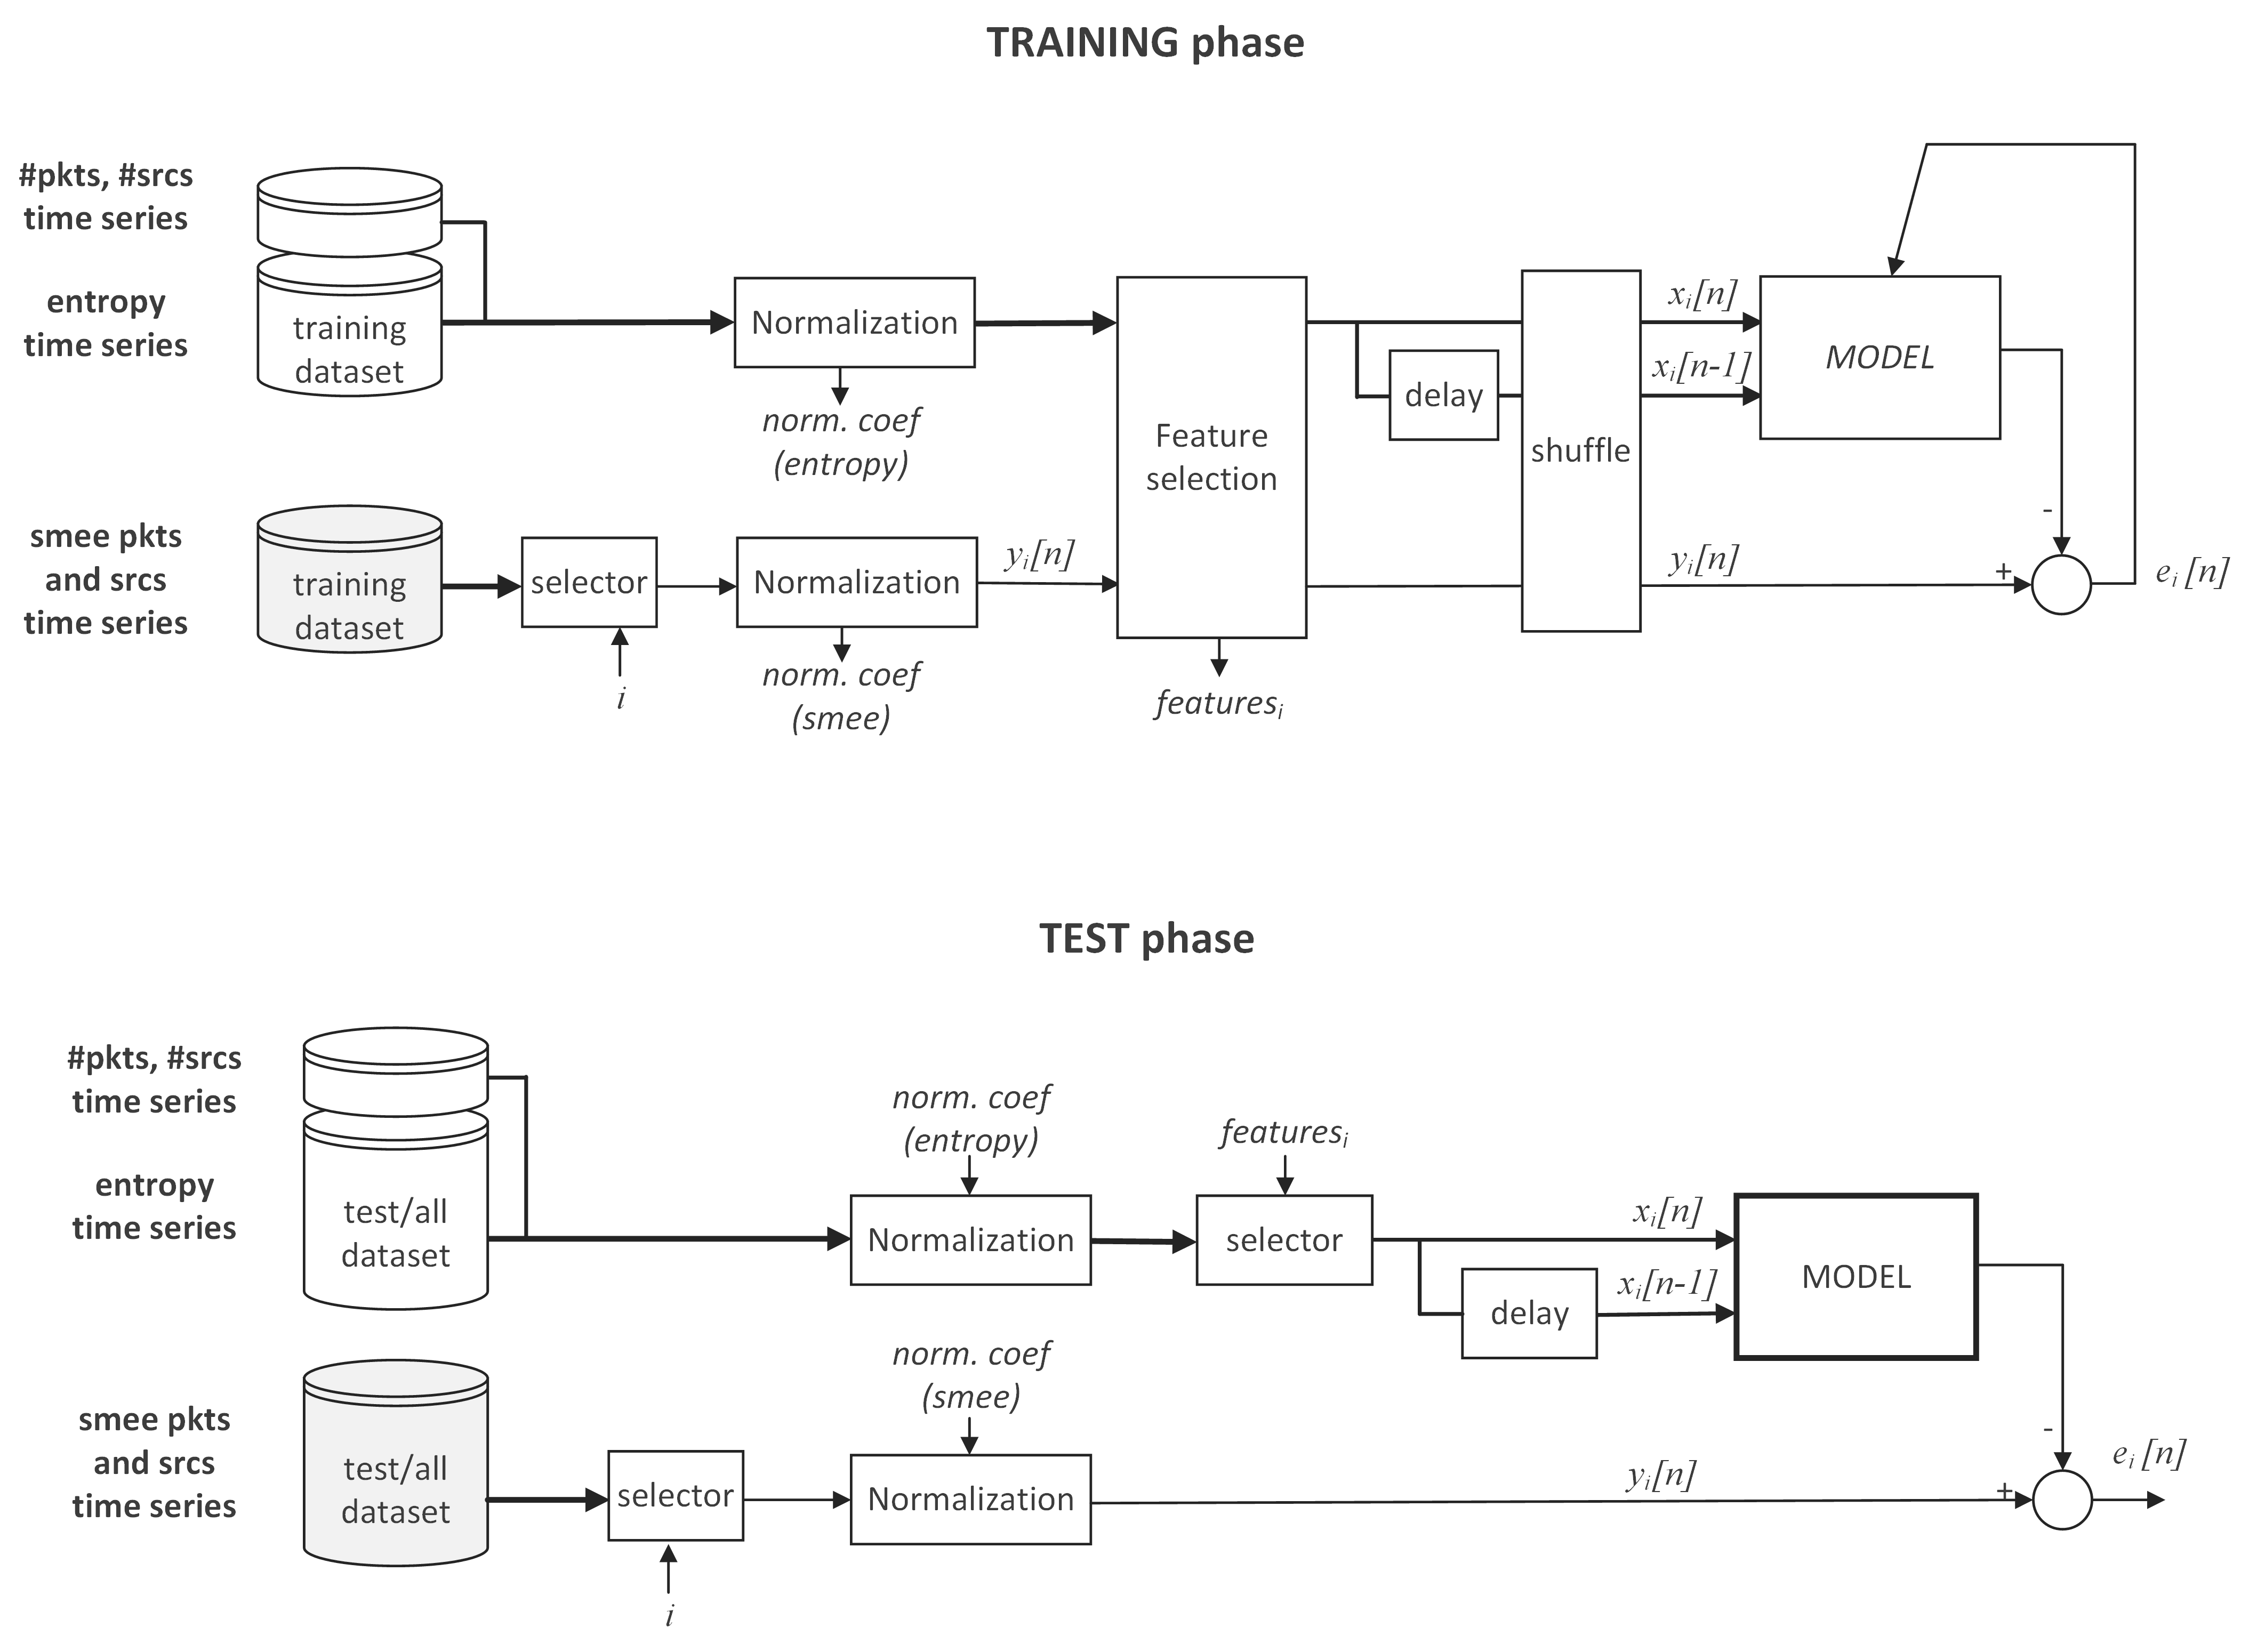
\includegraphics[width=0.95\linewidth]{graphics/modeling-example}
	\caption{Describe in the caption exactly what can be seen in the figure}
	\label{fig:modeling-example}
\end{figure}




\newpage